%\documentclass[twocolumn]{article}
\documentclass{report}

\usepackage{url}
\usepackage{indentfirst}
\usepackage{float}
\usepackage{listings} % Include the listings-package
\usepackage{mdframed}
\usepackage[numbers,sort]{natbib}
%\usepackage{titlesec} % Needed to support sub-subsections
%\usepackage[english]{babel} % Need for text wrap in table.
\usepackage{array} % Needed for centering in the table
\usepackage{graphicx}

% Defines the table of contents depth and the subsection numbering depth
\setcounter{secnumdepth}{5}
\setcounter{tocdepth}{5}

\title{\emph{HamSkill}: Run Haskell Anywhere \\
with ANTLR and Scala\\[1in]
	   CS252 Project Final Report}

\author{
  Zayd Hammoudeh \\
  (zayd.hammoudeh@sjsu.edu)
  }


\newcommand{\myparagraph}[1]{\paragraph{#1}\mbox{}\\}

% Skip lines after each paragraph.
\setlength\parskip{\baselineskip}

\begin{document}

\maketitle

\tableofcontents{\protect\newpage}

\renewcommand\thesection{\arabic{section}}
\section{Running in the Java Virtual Machine}\label{sec:jvm}

C is one of the most commonly used languages when the goal is maximum performance.  However, C/C++'s ``write once, compile anywhere" paradigm limits its portability.  In contrast, the near ubiquity of the Java Virtual Machine (JVM) allows Java to be "write once, run anywhere."  

On many occasions, developers have leveraged the JVM's ``run anywhere" capability to run allow other languages.  Examples include: JRuby for the Ruby programming language \cite{jruby}, Jython for the Python programming language \cite{jython_jvm}, Renjin for the R programming language \cite{renjin}, and Scala \cite{scala}.

Currently, there is no full implementation of Haskell in the JVM.  One Haskell dialect that is runnable in Java is Frege \cite{frege}.  

In this project, I will implement, \emph{HamSkill}, which is a transpiler from Haskell to Scala; \emph{HamSkill} enables a dialect of Haskell to be runnable in the JVM.  

\section{Key Project Requirements}\label{sec:keyProjectRequirements}

When designing and implementing this project, there were four primary goals:

\begin{itemize}

\item \textbf{Runnable in the Java Virtual Machine} - As explained in section~\ref{sec:jvm}, Java's Virtual Machine enables significant machine independence, which Haskell does not currently enjoy.

\item \textbf{Minimal JVM Requirements} - In addition to just running in the JVM, HamSkill was intended to be as standalone as possible.  For example, for most applications, it was not expected that the user would have Scala installed on their machine.  To achieve this, some advanced features may not be supported.

\item \textbf{Identical Input and Output Between Haskell and \emph{HamSkill}} - In many scenarios, it may not be sufficient for a program to run in Haskell and in JVM.  Rather, it may often be required that the generated output for the two programs be identical as well.  As such, \emph{HamSkill} will utilize an additional post processing step to ensure its output is identical to that generated by Haskell.

\item \textbf{Human Readable Output Code} - A transpiler is any program that takes source code from one programming languages and outputs as code in another programming language with a similar level of abstraction \cite{jansen_2015}.  To enable increased reuse of the outputted code, HamSkill will use proper indenting, newlines, etc. to maximize readability the generated output.  While this is not a requirement for the complete system to work properly, it can enhance the potential of the tool.

\end{itemize}

\section{\textit{HamSkill}'s Software Architecture}\label{sec:hamskillSoftwareArchitecture}

\emph{HamSkill} is a transpiler that takes input Haskell code, converts it to Scala, and then runs it in the JVM.  The \emph{HamSkill} implementation consists of four major components.  They are:

\begin{itemize}
   \item ANTLR Lexer and Parser
   \item Haskell Antlr Grammar
   \item HaskellMain Java Class
   \item Scala Runtime Environment
   \item ScalaOutput Antlr Grammar
   \item ScalaOutput Java Class
\end{itemize}

The relationships between these four components are shown in figure~\ref{fig:hamskillArchitecture}.

\begin{figure}[ht!]
	\centering
		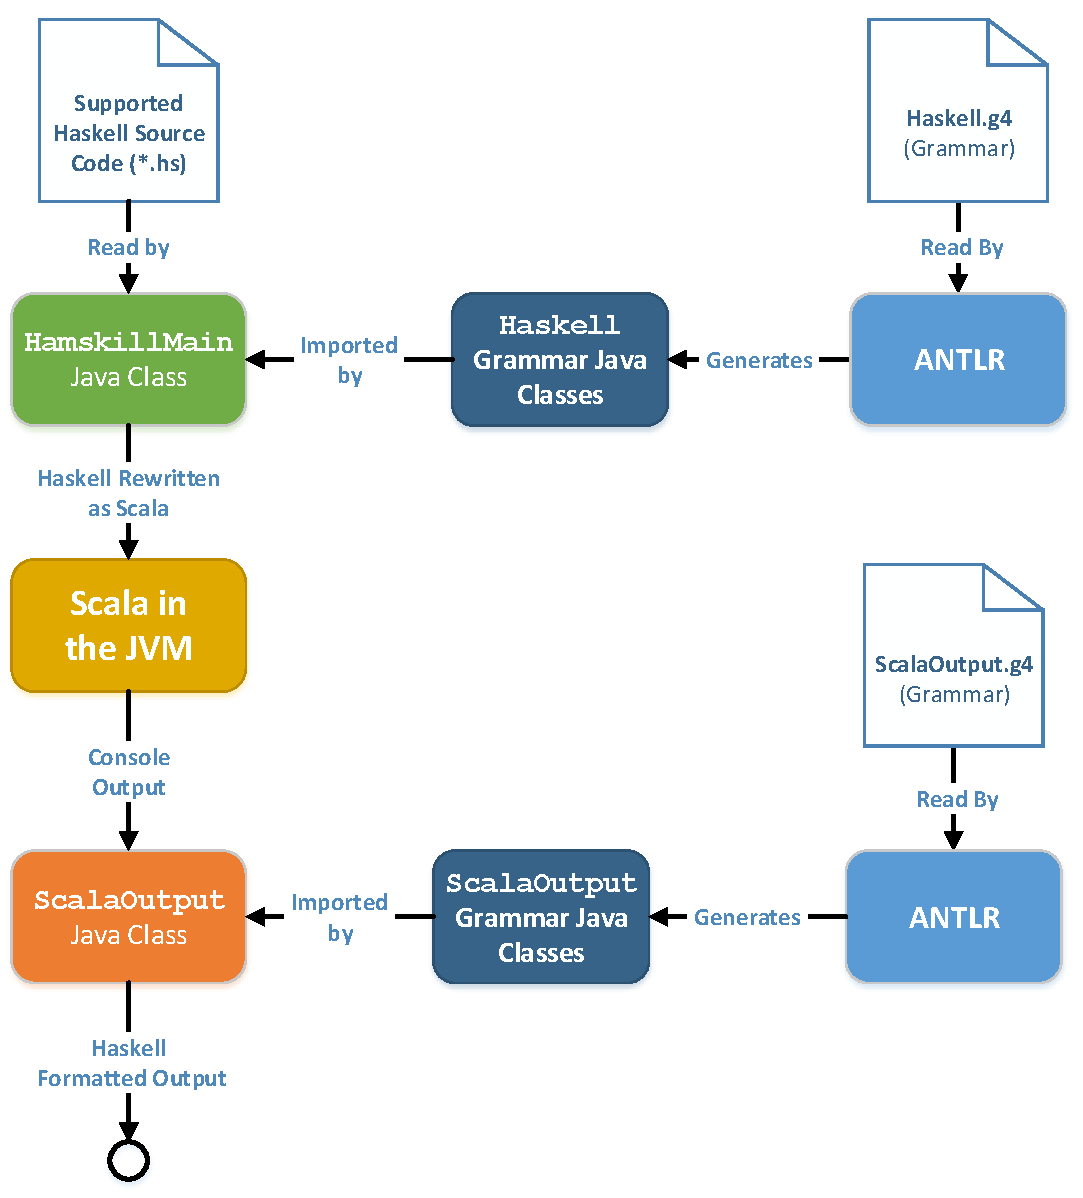
\includegraphics[width=1.0\textwidth]{images/cs252_project_diagram_cropped.pdf}
	\caption{HamSkill Project Architecture}
\end{figure}\label{fig:hamskillArchitecture}

The following subsections describe each of the components of this architecture.

\subsection{ANTLR}

ANTLR (\underline{AN}other \underline{T}ool for \underline{L}anguage \underline{R}ecognition) is an adaptive left-to-right, left-most deriviation (LL(*)) lexer and parser written in the Java programming language.  ANTLR's primary function is to read, parse, and process structured text (e.g. Haskell code) \cite{antlrDefinitiveReference}.  

\subsubsection{ANTLR Version 4 Grammar}

A grammar is a formal description of language; it is based off the concept of a context-free grammar in formal automata theory.  ANTLR version 4 (v4) grammar files (denoted by the file extension \emph{.g4}) explicitly define the how ANTLR will parse the structured text.  The grammar file may contain token definitions (which always start with a capital letter) and/or parser rules (which always start with a lowercase letter).  The tokens are groups of characters that form a single object; the parser then uses these tokens to recognize sentence structure within the document.

This project utilizes two separate grammars namely: \texttt{Haskell} and \texttt{ScalaOutput}.  They are described in the following two subsections.

\myparagraph{Haskell Grammar} 

The Haskell parsing grammar is stored in a file named "\texttt{Haskell.g4}."  This grammar defines both the tokens and abstract syntax tree for supported Haskell code.  Some of Haskell features it supports include:

\begin{itemize}
   \item \texttt{case} Statement
   \item \texttt{if}, \texttt{then}, \texttt{else} Conditional
   \item \texttt{Maybe} Monad
   \item Currying
   \item Partially Applied Functions
   \item Higher Order Functions
   \item Lazy Evaluation
\end{itemize}

For the complete feature set as well as specific Haskell syntax requirements, see section~\ref{sec:hamskillFeatures}.

\myparagraph{ScalaOutput Grammar} 

As mentioned in section~\ref{sec:keyProjectRequirements}, one of the key requirements of this project was that the outputs from Haskell and HamSkill should be identical.  Figure~\ref{fig:printListHaskell} and~\ref{fig:printListScala} show the code to print a list containing ``2", ``3", and ``4'' in Haskell and Scala respectively.  Note that the subsequent lines should the results of the print statement for the two languages are very different.

\begin{figure}[H]
\begin{mdframed}
\begin{lstlisting}[language=Haskell]
Prelude> putStrLn $ show [2, 3, 4]
[2,3,4]
\end{lstlisting}
\end{mdframed}
\caption{Printing a Three Element List in Haskell}\label{fig:printListHaskell}
\end{figure}

\begin{figure}[H]
\begin{mdframed}
\begin{lstlisting}[language=Scala]
scala> println(List(2,3,4))
List(2, 3, 4)
\end{lstlisting}
\end{mdframed}
\caption{Printing a Three Element List in Scala}\label{fig:printListScala}
\end{figure}

The \texttt{ScalaOutput} grammar (contained in the file "\texttt{Haskell.g4}") parses the output of the Scala program and converts it to a syntax that is more similar to that of Haskell.

\subsubsection{ANTLR Classes}

Programs that use ANTLR do not generally operate directly on the grammar.  Rather, the grammar is converted by ANTLR into a set of Java files; given an example grammar, \emph{GrammarName.g4},  ANTLR would create the following files:

\begin{itemize}
	\item \emph{GrammarName}Lexer.java - This class is the the lexer definition for the input grammar file.  It also extends ANTLR's base Lexer class.
	
	\item \emph{GrammarName}Parser.java - Each rule in the original grammar constitutes a method in this class; it forms the parser class definition for the input grammar file.
	
	\item \emph{GrammarName}.tokens - Assigns a token type (e.g. integer, identifier, floating point number etc.) to each token in the input grammar file.
	
	\item \emph{GrammarName}Listener.java \& \emph{GrammarName}BaseListener.java - ANTLR builds applies the grammar to a text input to build an Abstract Syntax Tree (AST).  While walking the tree, ANTLR fires events that can be captured by a listener\cite{antlrDefinitiveReference}.
\end{itemize}

Most programs that want to use ANTLR override the functions in the file \emph{GrammarName}BaseListener.java.


\myparagraph{HaskellTokensToScala}

\myparagraph{ScalaOutputTokensToHaskellFormat}


\subsection{Transpiler Output Language: Scala}

As mentioned previously, a transpiler takes source code from one programming language and converts it to code in another language.  It was also previous explained that the primary criteria when deciding on the output language was that it needed to be runnable in the Java Virtual Machine.  Other important criteria were:

\begin{itemize}

	\item \textbf{Higher Order Function Support} - Any language that is devoid of higher order support would not be a good match with a purely functional language like Haskell.
	
	\item \textbf{Similar Syntactic Structure} - Closer alignment between the input and output languages will simplify the trans-compilation.  Inevitably though, some amount of restructuring and reformatting will be required.  
	
	\item \textbf{Personal Interest} - Increased personal investment generally leads to a more fulfilling outcome for the student and a better project overall.  

\end{itemize}

The language that best fit all three of these criteria is Scala, which is a functional language which can be fully run inside the JVM \cite{whatIsScala}. What is more, it natively supports many of Haskell's core features including: functions written in a pattern matching style, immutability of objects, currying, partially applied functions, lazy evaluation, static typing, etc.  One of the disadvantages of Scala is its weaker type inference in comparison to Haskell; due to this specific requirements were placed on the requirements of the Haskell dialect supported by Hamskill as described in section \ref{sec:hamskillFeatures}.

It is also important to note that the author has had a personal predisposed interest in learning Scala given its extensive support by Apache Spark.  As such, given the "personal interest" requirement mentioned previously, the selection of Scala for this project became an even more obvious choice.

\myparagraph{\textit{HamSkill} Standard}

\myparagraph{\textit{HamSkill}+}

\section{HamSkill Features}\label{sec:hamskillFeatures}

This section enumerates the Haskell features that are supported by HamSkill.  It also describes any formatting requirements that may apply to these features.

\subsection{Immutability in Scala}\label{sec:immutabilityScala}

One of the key features of Haskell that allows it to achieve referential transparency is the immutability of data.  While it would be possible to develop an infrastructure in a language like Python to assure immutability, it is an encumbrance.  In cases such as this, it is almost always better to take advantage of a language's native features when possible.  In Scala, the {\tt val} construct ensure the immutability of an object without any user intervention.  For example, the code in figure~\ref{fig:scalaValConstruct} would raise a runtime error since it is trying to change the value of immutable data.

\begin{figure}[H]
\begin{mdframed}
\begin{lstlisting}[language=Scala]
val x = 5
x = 3
\end{lstlisting}
\end{mdframed}
\caption{Declaring Immutable Data in Scala}\label{fig:scalaValConstruct}
\end{figure}

\subsection{Lazy Evaluation}\label{sec:lazyEvaluationScala}

Another important aspect of Haskell is that it supports lazy evaluation.  This entails that data's value is not calculated until it is not needed.  Figure \ref{fig:lazyImmutabilityInScala} is an example of lazy evaluation with Scala as when this code is run, it will print a negative elapsed time (which is clearly not correct).

\begin{figure}[H]
\begin{mdframed}
\begin{lstlisting}[language=Scala]
def lazyTime(){
  lazy val t1 = System.nanoTime()
  val t2 = System.nanoTime()
  Thread.sleep(1000)
  println("Elapsed time is " + (t2-t1)/1000000 + "ms")
}
\end{lstlisting}
\end{mdframed}
\caption{Lazy, Immutable Code in Scala}\label{fig:lazyImmutabilityInScala}
\end{figure}

Scala also supports ``call-by-name" to achieve laziness of function parameters.  However, this feature is not truly lazy as it will recalculate the value each time the parameter is used in the function.  This limitation often degrades the overall the performance; for this reason, I do not plan to implement laziness in \emph{HamSkill} across functions.

\subsection{Supported Types}

\emph{HamSkill} will only support a select subset of Haskell's available types.  The list of planned types are: {\tt Bool}, {\tt Integer} (i.e. bounded), and {\tt List} (currently only finite lists are planned, but that may change depending on the complexity of the implementation).

While implementing floating point numbers would not add substantial complexity at a basic level, ensuring that the floating point behavior of \emph{HamSkill} (i.e. Scala) and Haskell are identical is beyond the scope of this project.

\subsection{Conversion from Functions to Methods}

The function in Haskell to convert data to string is ``{\tt show}". In contrast, the syntax in Scala to convert an object (e.g. ``x") to a string is ``{\tt x.toString()}".  Due to this, the ANTLR parser will need to be able to convert a prefix function to an object method call.

\subsection{Nested Function Calls}\label{sec:nestedFunctionCalls}

Imperative languages (e.g. Java) are generally more verbose than functional languages; Haskell is no exception to this.  Conciseness introduces significant challenges when writing a parser as the contextual information is reduced.  For example, figure \ref{fig:addTwoNumbersHaskell} is a simple line of Haskell code that prints to the screen the result of a function ``{\tt addTwoNumbs}" that takes two integers (e.g. ``{\tt x}" and ``{\tt y}") and sums them. 

\begin{figure}[H]
\begin{mdframed}
\begin{lstlisting}[language=Haskell]
putStrLn $ show $ addTwoNumbs x y
\end{lstlisting}
\end{mdframed}
\caption{Simple Function Call in \textbf{Haskell}}\label{fig:addTwoNumbersHaskell}
\end{figure}

Similar code in Java is shown in figure \ref{fig:addTwoNumbersJava}

\begin{figure}[H]
\begin{mdframed}
\begin{lstlisting}[language=Java]
System.out.println( addTwoNumbs(x, y) ) ;
\end{lstlisting}
\end{mdframed}
\caption{Simple Function Call in \textbf{Java}}\label{fig:addTwoNumbersJava}
\end{figure}

The Java syntax explicitly shows that {\tt addTwoInts} is a function since the parameters are inside parentheses and are comma separated.  To simplify the parsing for this in Haskell, the \emph{HamSkill} requires function arguments to be preceded and succeeded by triple parentheses ``\texttt{(((}" and ``\texttt{)))}".  Figure \ref{fig:addTwoNumbersHamSkill} shows the \emph{HamSkill} version of the Haskell code in figure \ref{fig:addTwoNumbersHamSkill}.

\begin{figure}[H]
\begin{mdframed}
\begin{lstlisting}[language=Haskell]
putStrLn $ show $ addTwoInts ((x y))
\end{lstlisting}
\end{mdframed}
\caption{Simple Function Call in \textbf{\emph{HamSkill}}}\label{fig:addTwoNumbersHamSkill}
\end{figure}

\subsection{Defining Scope and Scala Object Name via {\tt module}}

A program in Haskell is composed of a set of ``{\tt module}" files.  The ``{\tt module}" keyword is used to  scope of functions (e.g. {\tt public} or {\tt private}) as well as for defining an abstract data type \cite{haskellModule}.  In \emph{HamSkill}, I will use the Haskell module to define whether the Scala methods are private (since by default functions are {\tt public}) as well as the name of the Scala object.

\subsection{Partially Applied Functions}\label{sec:partiallyAppliedFunctions}

Haskell supports partially applied functions.  Figure \ref{fig:addFiveHaskell} shows the {\tt addTwoInts} function with a single argument (i.e. ``{\tt 5}") being stored in a variable ``{\tt addFive}".  

\begin{figure}[H]
\begin{mdframed}
\begin{lstlisting}[language=Haskell]
let addFive = addTwoInts 5
\end{lstlisting}
\end{mdframed}
\caption{Partially Applied addTwoInts Function in \textbf{Haskell}}\label{fig:addFiveHaskell}
\end{figure}

Partially applied functions in Scala have advantages and disadvantages in comparison to Haskell.  One of these disadvantages is evident when figures \ref{fig:addFiveHaskell} and \ref{fig:addFiveScala} are compared.  Note that the Scala function requires an underscore ("\_") for each missing argument as well as the type for that argument.  This makes converting Haskell code to Scala problematic as the function prototype must be fixed and known at conversion time.  

\begin{figure}[H]
\begin{mdframed}
\begin{lstlisting}[language=Scala]
val addFive = addTwoInts(5, _: Int)
\end{lstlisting}
\end{mdframed}
\caption{Partially Applied {\tt addTwoInts} Function in \textbf{Scala}}\label{fig:addFiveScala}
\end{figure}

To simplify this, \emph{HamSkill} will require that any partially defined functions are declared in the same file/module.  I will investigate using a predefined list of functions, but this may not be feasible or support will be very limited due to the requirement to define the parameter type.  What is more, partially applied functions will use need to use the "double parentheses style" described in section \ref{sec:nestedFunctionCalls}.

\subsection{Higher Order Function Support}\label{sec:higherOrderFunctions}

Scala and Haskell are both functional programming languages; one important consequence of this is that both support higher order functions.  \emph{HamSkill} will support functions as input parameters to functions.  If time allows, I will also investigate the ability to return functions from functions.  The extent to which this is supported will be dependent on the extent to which partially applied functions are supported as defined in section \ref{partiallyAppliedFunctions}.

\subsection{Haskell Lambda Function to Scala Anonymous Functions}\label{sec:lambdaAnonymousFunctions}

There is significant similarity between a Lamda function in Haskell and an anonymous function in Scala.  One primary difference is that Scala requires the developer to specify the types of the parameters in the anonymous function while Scala does not. For this project, I will implement support for anonymous functions either as parameters to other functions or for support for an operation such as folding or filtering a list. 

\subsection{Maybe Monad Support}

\section{\textit{HamSkill} Architecture}

Software testing is important for detecting defects in software programs.  What is more, there is different types of software testing including unit testing, module level testing, and system tests.  Given that ANTLR relies heavily on the Listener pattern, it reduces the ease at which unit testing can be performed.  What is more, given that \textit{HamSkill} relies on the end to end operation of programs written in Haskell, ANTLR, Java, and Scala, it really emphasizes the importance of system level test.

\subsection{System Level and Regression Testing via Use Cases}



\subsection{Testbench Implementation Overview}

The \textit{HamSkill} test architecture is written as a \texttt{bash} script (see the file in the submission \path{Test_Bench/test_bench.sh}.  The function ``\texttt{perform\_hamskillStd\_and\_hamskillPlus\_test}" is the most important in the script as it is responsible for performing most of the test; the basic operational flow of this function is:

\begin{itemize}

\item \textbf{Step \#1}: The function is provided the name of a Haskell program written in the dialect supported by \textit{HamSkill}, but without the file extension.

\item \textbf{Step \#2}: The Haskell program is run in Haskell, and the program's output is stored to a specific file on disk using the \texttt{bash} command ``\texttt{>}". 

\item\label{item:runHamskillStandard} \textbf{Step \#3}: Run Hamskill in standard mode and store the results to a file using the bash command ``\texttt{>}". 

\item\label{item:diffHamskillStandard} \textbf{Step \#4}: Perform a file difference operation (using the \texttt{bash} \texttt{diff} command) on the output files from Haskell and HamSkill standard.  If the two files are identical, then mark the test as passing; if they are different, the test fails.
 
\item \textbf{Step \#5}: Repeat steps \#~\ref{item:runHamskillStandard} and \#~{item:diffHamskillStandard} using \texttt{HamSkill+}.

\end{itemize}

\pagebreak
\bibliographystyle{plainurl}
\bibliography{final_report_biblio}

\end{document}
